\section{Graph Neural Network Based Approaches}

\begin{frame}[t]{Node Embedding}\vspace{10pt}
    Each node can be identified with a vector.\vspace{20pt}
    
    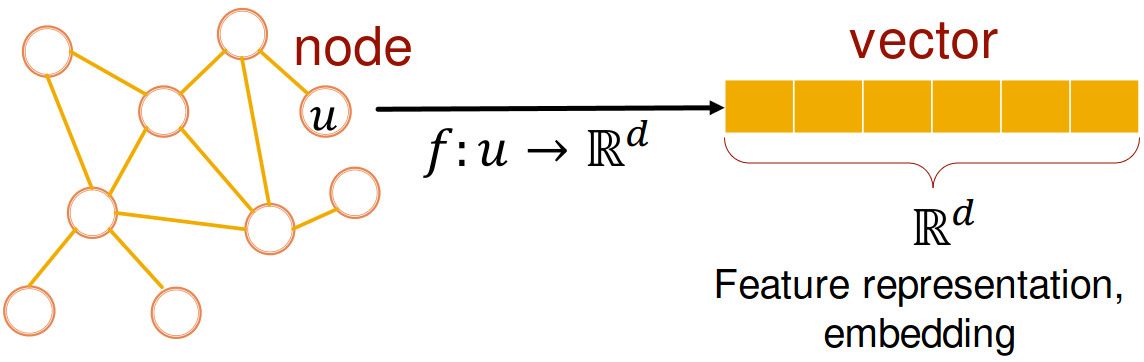
\includegraphics[scale=.26]{nodeEmbeddingGoal}
\end{frame}

\begin{frame}[t]{Embedding Goals}

    \begin{block}{Task: Map nodes into an embedding space}
    
        \begin{itemize}
        
            \item Similarity of embeddings between nodes indicates their similarity in the network. For example: Both nodes are close to each other (connected by an edge)

            \item Encode network information
            
            \item Potentially used for many downstream predictions
        \end{itemize}
        
    \end{block}

    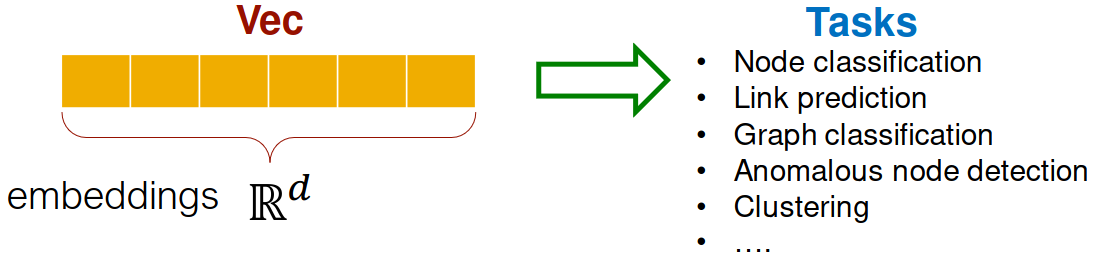
\includegraphics[scale=.33]{nodeEmbeddingTasks}
    
\end{frame}

\begin{frame}[t]{Example Node Embedding}
    2D embedding of nodes of the Zachary’s Karate Club network:\\ \vspace{20pt}
    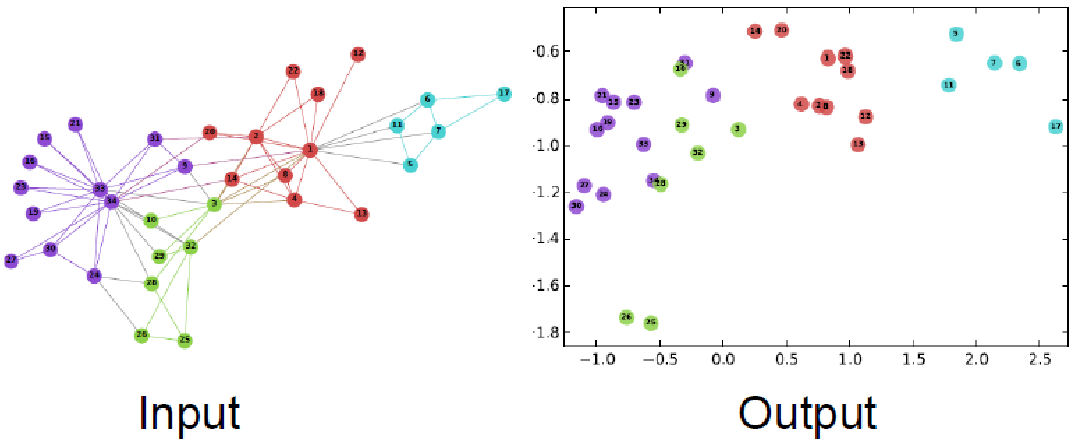
\includegraphics[scale=.3]{images/Zakarys2DExample.png}
\end{frame}

\begin{frame}[t]{Word2Vec}
    \only<1>{
        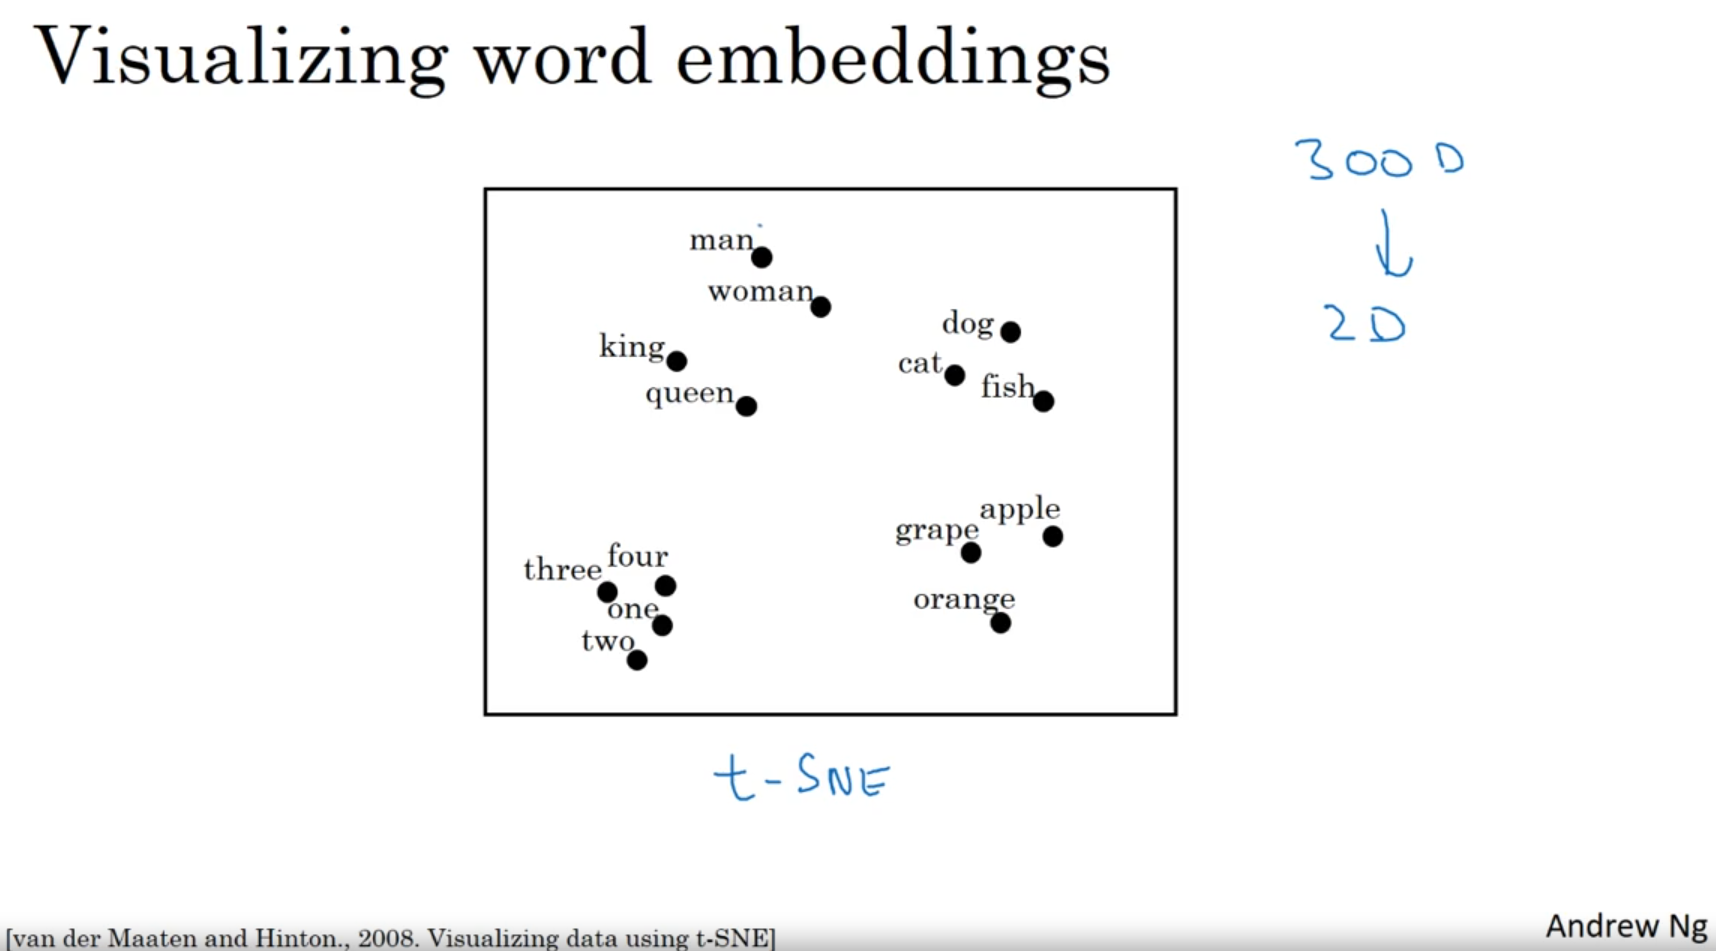
\includegraphics[scale=.18]{images/VisualizeWordEmbeddingWord2Vec.png}
        \unfootnote{
            \href{https://towardsdatascience.com/nlp-101-word2vec-skip-gram-and-cbow-93512ee24314}{NLP 101: Word2Vec — Skip-gram and CBOW}\\
            \href{http://cs224d.stanford.edu/lecture_notes/notes1.pdf}{Lecture notes CS224D: Deep Learning for NLP Part-I}\\
            \href{https://www.coursera.org/learn/nlp-sequence-models/home/week/2}{Coursera - Andrew Ng - Sequence Model - Week 2}
        }
    }
    \only<2>{
        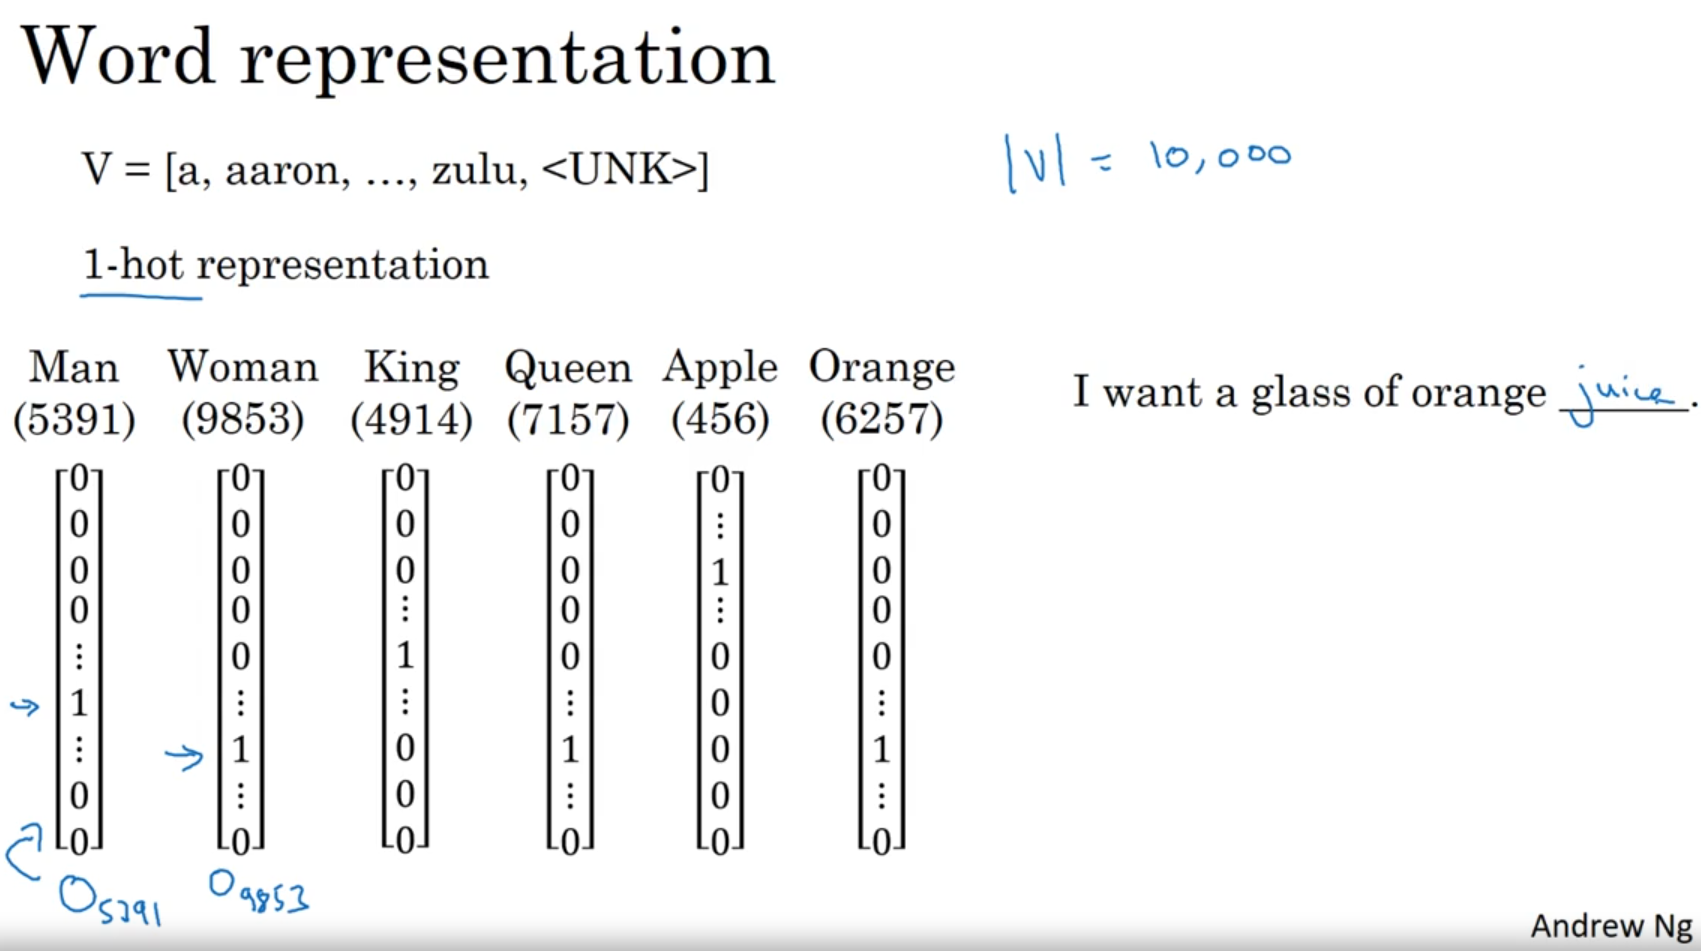
\includegraphics[scale=.18]{images/WordRepresentationOfWord2Vec.png}
    }
    \only<3>{
        \begin{block}{CBOW Objective}
            We want to predict the target from the context.
        \end{block}
        The \boldblue{brown fox} \boldred{jumped} \boldblue{over the} lazy dog.
        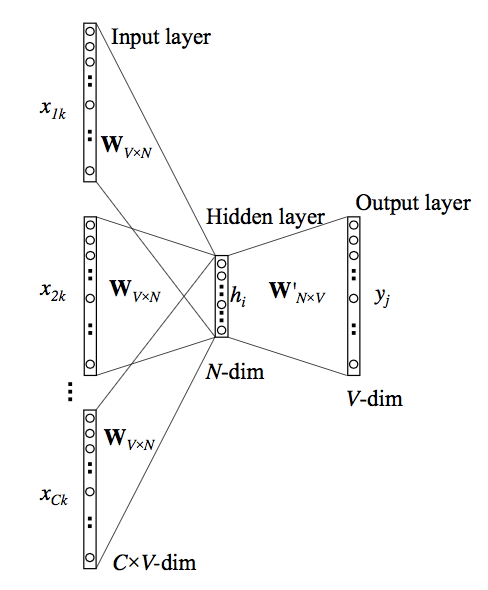
\includegraphics[scale=.29]{CBOWWord2Vec}

    }
\end{frame}

\begin{frame}[t]{DeepWalk}
    \unfootnote{
        \href{https://towardsdatascience.com/deepwalk-its-behavior-and-how-to-implement-it-b5aac0290a15}{DeepWalk: Its Behavior and How to Implement It}
    }

    \begin{itemize}
        \item For each node, perform N “random steps” starting from that node
        \item Treat each walk as a sequence of node-id strings
        \item Given a list of these sequences, train a word2vec model using the Skip-Gram algorithm on these string sequences
    \end{itemize}

    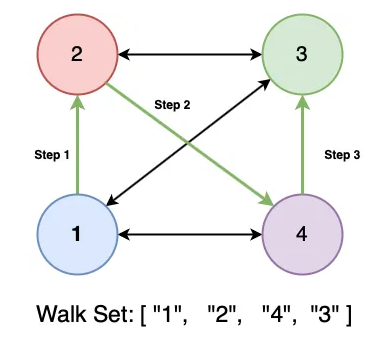
\includegraphics[scale=.33]{images/DeepWalkRandomWalk.png}
\end{frame}

\begin{frame}[t]{Node2Vec}
    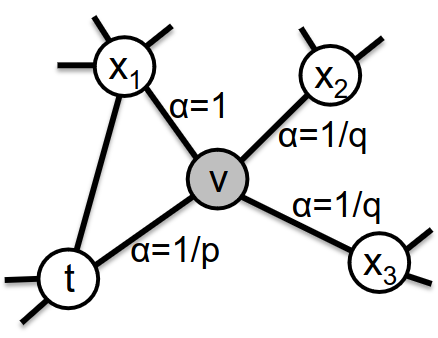
\includegraphics[scale=.35]{Node2VecExploration}

    \boldblue{Biased random walk to explore more like DFS or BFS}
\end{frame}